%!TEX root = ../dissertation.tex

\chapter{Introduction}
\label{chapter:introduction}
The Internet of Things \gls{IoT} can be seen as a web of interconnected devices that go from everyday wearable objects into fully deployed sensor networks. Despite the huge variety and characteristics of these devices, one thing that they all have in common is the constrained nature that they are built upon. In order to enable the massive deployment to be expected in the near future,\footnote{http://blogs.wsj.com/cio/2015/06/02/internet-of-things-market-to-reach-1-7-trillion-by-2020-idc/} \gls{IoT} devices must be accessible and affordable, capable of operating under lossy wireless networks while being battery powered. This poses a challenge to current Internet protocols since the assumptions regarding the devices' capabilities and objectives do not hold true.\\ To allow the \gls{IoT} vision to come forward, several new protocols have been developed across the OSI layers, each addressing and tackling the challenges involved in trying to keep the quality and assurances of stronger, more expensive protocols, on constrained systems. After being thoroughly analysed, these protocols have been selected and grouped in a power-efficient stack, establishing a base line for power consumption.
Additionally, major attention has been given to information security because for both corporations and individuals, the interconnection of the devices around us can provide information about our choices and whereabouts, therefore leaking corporate information or simply reducing our individual privacy \cite{Ukil2015}. Thus, the focus moved towards adding mechanism to ensure authentication, confidentiality and integrity of the transmitted information by securing the communication channel. In order to understand the cost of adding these mechanisms, additional experiments have been performed so that the added power consumption can be measured, profiled and documented, enabling the finding of the best parameters and requirements for a desired level of security.\\

TODO: não tive inspiração suficiente, ainda, para escrever um paragrafo que diga que construimos uma solução assente num cenário smart campus porque é um bom modelo para testarmos o sistema e obtermos medições interessantes, e que também foi dado grande foco na facilidade de uso e monitorização do sistema, permiting a qualquer um sem conhecimentos técnicos fazer deploy da rede de sensores e monitorizar os valores reportados

\section{Document Roadmap}

In this document we start by analysing the state-of-the-art in Section \ref{sec:related_work}. This includes the selection of the most adequate protocol stack for our necessities in Section \ref{sec:protocol_analysis}, an overview of the existing attacks and mitigation strategies in Section \ref{sec:attack_analysis} and a summary of the existing solutions regarding secure insertion of new nodes in an existing network in Section \ref{sec:secure_bootstrapping}. All this knowledge will be integrated into our proposed solution defined in Section \ref{sec:proposed_solution}. Section \ref{sec:work_evaluation} defines how our work will be tested and evaluated so that a power-aware perspective can be achieved. Section \ref{sec:work_planning} states how the development of our solution will unwind over the next months and finally, Section \ref{sec:conclusion} presents the conclusion of this document.

\section{Environment Overview}
\label{sec:network_overview}
There are many applicability domains and different methods for creating \gls{IoT} networks. 
Some provide direct connectivity of nodes to the Internet while others provide a common gateway for interfacing with external networks. 
In our work, we focus on scenarios where network nodes are not directly connected to the Internet and require additional network components for proper communication as depicted in Figure \ref{fig:net_overview}.

\begin{figure}[h]
  \centering
  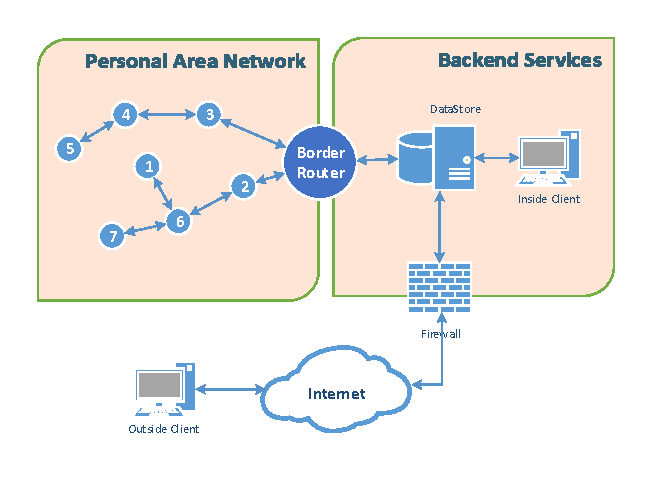
\includegraphics[width=0.8\linewidth]{figures/Network_Overview.pdf}
  \caption{IoT Network Overview.}
  \label{fig:net_overview}
\end{figure}

In this type of architectures, the sensing or actuating nodes belong to a very constrained network with specific protocols and header compression mechanisms, requiring an interface device -- the border router -- in order to communicate with external networks.
After reaching the external network, incoming messages are processed to convert sensor data into useful information which is then stored or used to trigger events. 
This information can then be accessed by users either on the same network or by making requests through the Internet. 

This type of deployment could be used, for example, in a home intrusion system or in a factory monitoring system. 
In the home intrusion system scenario, the network nodes would create a sensor network that propagates events in the case of an intrusion and the additional infrastructure would be in charge of receiving these events and notifying the police authorities. 
In the factory monitoring system scenario, the network nodes would create a sensor network that would be permanently reporting up-to-date readings of machinery control values like: temperature, pressure and power; 
and the additional infrastructure would in charge of supplying this information to a dashboard for the factory workers. 
If an attacker could disable these systems, he could then 
%rob the house or 
cause an emergency shut-down of the factory machinery due to lack of control over the working conditions. 
These are real concerns backed by a range of attacks that focuses on disabling \gls{IoT} networks by placing the nodes offline. These attacks are presented in the following Section.